\documentclass[tikz,border=8pt]{standalone}
% Shared look for every TikZ diagram. Load with % Shared look for every TikZ diagram. Load with % Shared look for every TikZ diagram. Load with \input{../../tools/tikz-style.tex}
\usepackage[T1]{fontenc}
\usepackage{lmodern}
\renewcommand{\sfdefault}{lmr}  % diagrams use the same serif as the text
\usetikzlibrary{arrows.meta, positioning, shapes.geometric, calc, fit, backgrounds}
\definecolor{cblue}{HTML}{4C78A8}
\definecolor{corange}{HTML}{F58518}
\definecolor{cgreen}{HTML}{54A24B}
\definecolor{cred}{HTML}{E45756}
\definecolor{cpurple}{HTML}{B279A2}
\definecolor{cgrey}{HTML}{6B6B6B}
\tikzset{
  every picture/.style={font=\sffamily, line width=1.2pt},
  box/.style={draw=#1, fill=#1!12, rounded corners=4pt, align=center, inner sep=7pt, minimum height=1.1cm},
  box/.default=cgrey,
  arrow/.style={-{Stealth[length=3mm]}, draw=cgrey, line width=1.4pt},
  title/.style={font=\sffamily\bfseries\Large},
  note/.style={font=\sffamily\small, text=cgrey, align=center},
}
\AtBeginDocument{\hyphenpenalty=10000 \exhyphenpenalty=10000}

\usepackage[T1]{fontenc}
\usepackage{lmodern}
\renewcommand{\sfdefault}{lmr}  % diagrams use the same serif as the text
\usetikzlibrary{arrows.meta, positioning, shapes.geometric, calc, fit, backgrounds}
\definecolor{cblue}{HTML}{4C78A8}
\definecolor{corange}{HTML}{F58518}
\definecolor{cgreen}{HTML}{54A24B}
\definecolor{cred}{HTML}{E45756}
\definecolor{cpurple}{HTML}{B279A2}
\definecolor{cgrey}{HTML}{6B6B6B}
\tikzset{
  every picture/.style={font=\sffamily, line width=1.2pt},
  box/.style={draw=#1, fill=#1!12, rounded corners=4pt, align=center, inner sep=7pt, minimum height=1.1cm},
  box/.default=cgrey,
  arrow/.style={-{Stealth[length=3mm]}, draw=cgrey, line width=1.4pt},
  title/.style={font=\sffamily\bfseries\Large},
  note/.style={font=\sffamily\small, text=cgrey, align=center},
}
\AtBeginDocument{\hyphenpenalty=10000 \exhyphenpenalty=10000}

\usepackage[T1]{fontenc}
\usepackage{lmodern}
\renewcommand{\sfdefault}{lmr}  % diagrams use the same serif as the text
\usetikzlibrary{arrows.meta, positioning, shapes.geometric, calc, fit, backgrounds}
\definecolor{cblue}{HTML}{4C78A8}
\definecolor{corange}{HTML}{F58518}
\definecolor{cgreen}{HTML}{54A24B}
\definecolor{cred}{HTML}{E45756}
\definecolor{cpurple}{HTML}{B279A2}
\definecolor{cgrey}{HTML}{6B6B6B}
\tikzset{
  every picture/.style={font=\sffamily, line width=1.2pt},
  box/.style={draw=#1, fill=#1!12, rounded corners=4pt, align=center, inner sep=7pt, minimum height=1.1cm},
  box/.default=cgrey,
  arrow/.style={-{Stealth[length=3mm]}, draw=cgrey, line width=1.4pt},
  title/.style={font=\sffamily\bfseries\Large},
  note/.style={font=\sffamily\small, text=cgrey, align=center},
}
\AtBeginDocument{\hyphenpenalty=10000 \exhyphenpenalty=10000}

\begin{document}
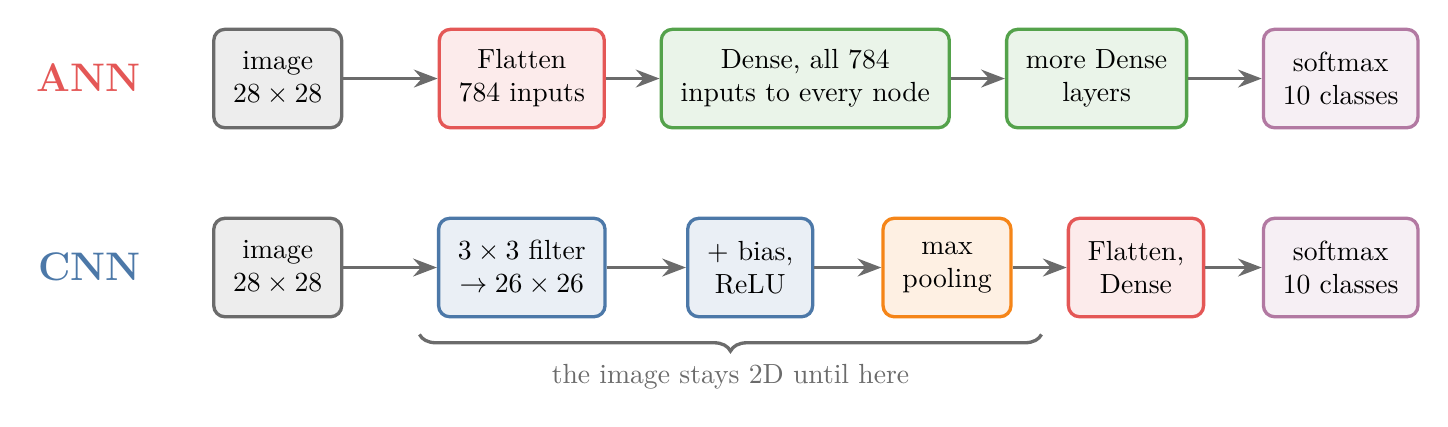
\begin{tikzpicture}[s/.style={box=#1, minimum height=1.25cm, font=\sffamily\normalsize, align=center}, s/.default=cgrey]
  \node[title, anchor=east, text=cred] at (-0.4,0) {ANN};
  \node[s] (a0) at (1.2,0) {image\\$28\times28$};
  \node[s=cred] (a1) at (4.3,0) {Flatten\\784 inputs};
  \node[s=cgreen] (a2) at (7.9,0) {Dense, all 784\\inputs to every node};
  \node[s=cgreen] (a3) at (11.6,0) {more Dense\\layers};
  \node[s=cpurple] (a4) at (14.7,0) {softmax\\10 classes};
  \foreach \x/\y in {a0/a1,a1/a2,a2/a3,a3/a4} \draw[arrow] (\x) -- (\y);
  \node[title, anchor=east, text=cblue] at (-0.4,-2.4) {CNN};
  \node[s] (c0) at (1.2,-2.4) {image\\$28\times28$};
  \node[s=cblue] (c1) at (4.3,-2.4) {$3\times3$ filter\\$\rightarrow 26\times26$};
  \node[s=cblue] (c2) at (7.2,-2.4) {+ bias,\\ReLU};
  \node[s=corange] (c3) at (9.7,-2.4) {max\\pooling};
  \node[s=cred] (c4) at (12.1,-2.4) {Flatten,\\Dense};
  \node[s=cpurple] (c5) at (14.7,-2.4) {softmax\\10 classes};
  \foreach \x/\y in {c0/c1,c1/c2,c2/c3,c3/c4,c4/c5} \draw[arrow] (\x) -- (\y);
  \draw[decorate, decoration={brace, amplitude=6pt, mirror}, cgrey] (3.0,-3.25) -- (10.9,-3.25)
    node[midway, below=7pt, note, font=\sffamily\normalsize] {the image stays 2D until here};
\end{tikzpicture}
\end{document}
